\documentclass{beamer}
\usepackage{../common_slides}
\usepackage{tikz-qtree}
\usepackage{pdfpages}

\title{Convolutional Networks 1}
\date{}
\author{CS 287}

\usepackage{stackengine}
\stackMath
\newlength\matfield
\newlength\tmplength
\def\matscale{1.}
\newcommand\dimbox[3]{%
  \setlength\matfield{\matscale\baselineskip}%
  \setbox0=\hbox{\vphantom{X}\smash{#3}}%
  \setlength{\tmplength}{#1\matfield-\ht0-\dp0}%
  \fboxrule=1pt\fboxsep=-\fboxrule\relax%
  \fbox{\makebox[#2\matfield]{\addstackgap[.5\tmplength]{\box0}}}%
}
\newcommand\raiserows[2]{%
   \setlength\matfield{\matscale\baselineskip}%
   \raisebox{#1\matfield}{#2}%
}
\newcommand\matbox[4]{
  \stackunder{\dimbox{#1}{#2}{$#4$}}{\scriptstyle #3}%
}

\begin{document}

\begin{frame}
  \titlepage
\end{frame}

\begin{frame}{Review: NGram Issues}
  
  In training we might see, 

  \begin{center}
    the arizona corporations commission \alert{authorized}
  \end{center}

  But at test we see, 
  \begin{center}
    the colorado businesses organization \alert{\_\_\_}
  \end{center}
  \pause 
  
  \begin{itemize}
  \item Does this training example help here?
    \begin{itemize}
    \item Not really. No count overlap.
    \end{itemize}
    \air 
    \pause 
  \item Does backoff help here? 
    \begin{itemize}
    \item Maybe, if we have seen organization.
    \item Mostly get nothing from the earlier words.
    \end{itemize}
  \end{itemize}
\end{frame}


\begin{frame}{Review: A Neural Probabilistic Language Model }  
  Optional, direct connection layers,

  \[NN_{DMLP1}(\boldx) =  [\tanh(\boldx\boldW^1 + \boldb^1), \boldx] W^2 + \boldb^2\]

  \begin{itemize}
  \item $\boldW^1 \in \reals^{\din \times \dhid}, \boldb^1 \in \reals^{1 \times \dhid}$; first affine transformation
  \item $\boldW^2 \in \reals^{(\dhid + \din)  \times \dout}, \boldb^2 \in \reals^{1 \times \dout}$; second affine transformation
  \end{itemize}
\end{frame}

\begin{frame}{Review: A Neural Probabilistic Language Model (Bengio, 2003)}  
  \begin{center}
    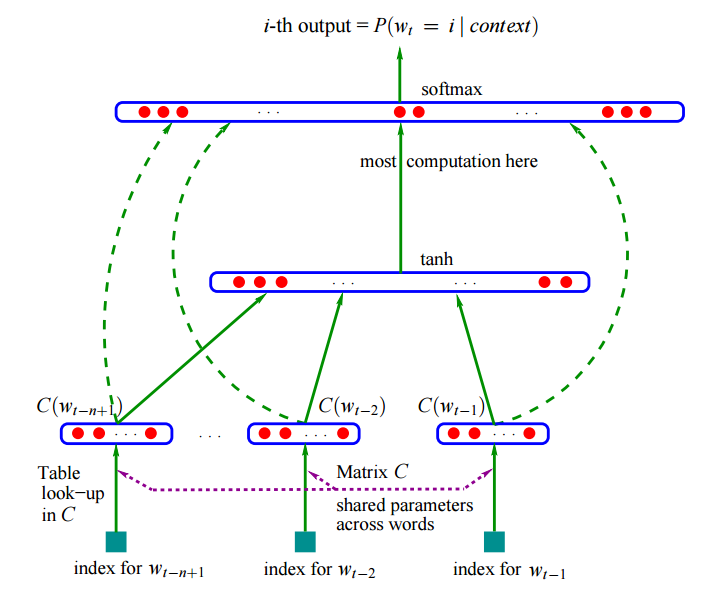
\includegraphics[width=7cm]{bengio}
  \end{center}
  Dashed-lines show the optional direct connections, $C = v$.
\end{frame}


\begin{frame}{Review: Comparison}
  Both count-based models and feed-forward NNLMs are Markovian language models, 

  Comparison:
  \begin{itemize}
  \item Training Speed: ngrams are much faster (more coming)
  \item Usage Speed: ngrams very fast, NN can be fast with some tricks. 
  \item Memory: NN models can be much smaller (but there are big ones)
  \item Accuracy: Comparable for small data, NN does better with more.
  \end{itemize}
  
  Advantages of NN model
  \begin{itemize}
  \item Can be trained end-to-end.
    \air 
  \item Does not require smoothing methods.
  \end{itemize}

  % \alert{NGram Models}
  % \begin{itemize}
  % \item Fast to train
  % \item Can 
  % \end{itemize}

  % \structure{Neural Models}
  % \begin{itemize}
  % \item Slower to train
  % \item
  % \end{itemize}
\end{frame}


\begin{frame}{Quiz}

Neural language models can be poor at assigning very high probability
to high confidence decisions, for instance \texttt{major league baseball}
or \texttt{united states of america}. 

\air 

\begin{itemize}
\item Give a high-level explanation of why this might occur compared to an n-gram 
model.
\item  Describe a variant of the Bengio model that is able to incorporate extra parameters 
to allow for rare cases that should have high probability.  
\end{itemize}
\end{frame}


\section{Text Classification Review}


\begin{frame}{Sentiment}
  \structure{Good Sentences}
  \begin{itemize}
  \item   A thoughtful, provocative, insistently humanizing film. 
  \item   Occasionally melodramatic, it's also extremely effective.
    \item   Guaranteed to move anyone who ever shook, rattled, or rolled.   
  \end{itemize}

  \alert{Bad Sentences}
  \begin{itemize}
  \item A sentimental mess that never rings true.  
  \item This 100-minute movie only has about 25 minutes of decent material.
  \item Here, common sense flies out the window, along with the hail of
    bullets, none of which ever seem to hit Sascha.
  \end{itemize}
\end{frame}



\begin{frame}{Review Linear Models for Classification}
  Linear model,
  \[\hat{\boldy} = f(\boldx \boldW + \boldb)\]
  \begin{itemize}
  \item $\boldW \in \reals^{\din \times \dout}, \boldb \in \reals^{1 \times \dout}$; model parameters
  \item $f: \reals^{\dout} \mapsto \reals^{\dout}$; activation function
  \item Sometimes $\boldz = \boldx \boldW + \boldb$ informally ``score'' vector.
  \item Note $\boldz$ and $\hat{\boldy}$ are not one-hot.
  \end{itemize}

  \air

  Class prediction,
  \[ \hat{c} = \argmax_{i \in \mcC} \hat{y_i}  = \argmax_{i \in \mcC} (\boldx \boldW + \boldb)_i    \]
\end{frame}

\begin{frame}{Features 1: Sparse Bag-of-Words Features}
  Representation is counts of input words, 
  \begin{itemize}
  \item $\mcF$; the vocabulary of the language.
  \item $\boldx = \sum_{i} \bolddelta(f_i)$ 
  \end{itemize}

  Example: Movie review input, 
  \begin{center}
    \texttt{A sentimental mess}
    \begin{eqnarray*}
      \boldx &=& \bolddelta(\texttt{word:A}) + \bolddelta(\texttt{word:sentimental}) \\ 
    &+& \bolddelta(\texttt{word:mess})
    \end{eqnarray*}

    \[ \boldx^\top =\begin{bmatrix} 1 \\ \vdots
        \\ 0\\ 0 \\ \end{bmatrix} +\begin{bmatrix} 0 \\
        \vdots \\ 0\\ 1 \\ \end{bmatrix} +
     \begin{bmatrix} 0 \\ \vdots \\ 1\\ 0 \\ \end{bmatrix} 
    =\begin{bmatrix} 1 \\ \vdots \\ 1 \\ 1 \\ \end{bmatrix} 
    \begin{matrix*}[l] \mathrm{\texttt{word:A}} \\ \vdots \\ \mathrm{\texttt{word:mess}} \\ \mathrm{\texttt{word:sentimental}} \\ \end{matrix*}
     \]
  \end{center}
\end{frame}


\begin{frame}{Features 2: Sparse Bag-of-Bigrams Features}
  Representation is counts of input bigrams, 
  \begin{itemize}
  \item $\mcF$; the vocabulary of the bigram language.
  \item $\boldx = \sum_{i} \bolddelta(f_i)$ 
  \end{itemize}

  Example: Movie review input, 
  \begin{center}
    \texttt{A sentimental mess}
    \begin{eqnarray*}
      \boldx &=& \bolddelta(\texttt{word:A})+ \bolddelta(\texttt{bigram:A:sentimental}) \\
      &+&  \bolddelta(\texttt{word:sentimental}) +   \bolddelta(\texttt{bigram:sentimental:mess})  \\
      &+& \bolddelta(\texttt{word:mess})
    \end{eqnarray*}

    
  \end{center}
\end{frame}




\begin{frame}{Features 3: Continuous Bag-of-Words Features}
  \[ \boldx = \sum_{i=1}^{k} v(f_i; \theta) = \sum_{i=1}^{k} \bolddelta(f_i) \boldW^0\]

  \begin{itemize}
  \item $\mcF$; the vocabulary of the language.
  \item $\boldx = \sum_{i} \bolddelta(f_i)$ 
  \end{itemize}

  Example: Movie review input, 
  \begin{center}
    \[\boldx = v(\texttt{word:A}) + v(\texttt{word:sentimental}) + v(\texttt{word:mess})\]
    \[ \boldx^\top = \begin{bmatrix} 0.2 \\ \vdots \\ 1.2 \\ -0.5 \\ \end{bmatrix} + \begin{bmatrix} 0.8 \\ \vdots \\ 1.0\\ -1.0 \\ \end{bmatrix} +
     \begin{bmatrix} 0.1 \\ \vdots \\ 9.2 \\ -2.0 \\ \end{bmatrix} 
    =  \begin{bmatrix} 1.1 \\ \vdots \\ 11.4 \\ -3.5 \\ \end{bmatrix} 
     \]
    % \begin{matrix*}[l]  \vdots \\  \mathrm{\texttt{word:A}} + \mathrm{\texttt{word:mess}} + \mathrm{\texttt{word:sentimental}} \\  \\ \end{matrix*}
  \end{center}
\end{frame}

\begin{frame}{Features 4: Continuous Bag-of-Bigrams Features?}
  Representation is counts of input bigrams, 
  \begin{itemize}
  \item $\mcF$; the vocabulary of the bigram language.
  \item $\boldx = \sum_{i} \bolddelta(f_i)$ 
  \end{itemize}

  Example: Movie review input, 
  \begin{center}
    \texttt{A sentimental mess}
    \begin{eqnarray*}
      \boldx &=& v(\texttt{word:A})+ v_2(\texttt{bigram:A:sentimental}) \\
      &+&  v(\texttt{word:sentimental}) +   v_2(\texttt{bigram:sentimental:mess})  \\
      &+& v(\texttt{word:mess})
    \end{eqnarray*}

  \end{center}
\end{frame}

\begin{frame}{Neural Network}
  One-layer multi-layer perceptron architecture,

  \[NN_{MLP1}(\boldx) =  g(\boldx\boldW^1 + \boldb^1)W^2 + \boldb^2\]
  \begin{itemize}
  \item $\boldx\boldW + \boldb$; \textit{perceptron}
  \item $\boldx$ is the dense representation in $\reals^{1 \times \din}$
  \item $\boldW^1 \in \reals^{\din \times \dhid}, \boldb^1 \in \reals^{1 \times \dhid}$; first affine transformation
  \item $\boldW^2 \in \reals^{\dhid \times \dout}, \boldb^2 \in \reals^{1 \times \dout}$; second affine transformation
  \item $g:\reals^{\dhid \times \dhid}$ is an \textit{activation non-linearity} (often pointwise)
  \item $g(\boldx\boldW^1 + \boldb^1)$ is the \textit{hidden layer}
  \end{itemize}
\end{frame}
\section{Convolutions} 

\begin{frame}{Windowed Classification}
  Alternative method, windows into MLP.

  \textbf{Goal:} predict $t_5$.


  \begin{itemize}
  \item Windowed word model.

  \[ w_1\ w_2\ [\textcolor{red}{w_3\ w_4\ w_5\ w_6\ w_7}]\ w_8 \]

  \item $w_3, w_4$; left context
  \item $w_5$; Word of interest
  \item $w_6, w_7$; right context

  \item $\dwin$; size of window ($\dwin = 5$)
  \end{itemize}
\end{frame}



\begin{frame}{All Window for Classification}
  \textbf{Idea:} Use window at each location. 

  
     \[ [\textcolor{red}{w_1 \ w_2\ w_3\ w_4\ w_5}]\ w_6\ w_7\ w_8 \]
     \[ w_1\ [\textcolor{red}{w_2\ w_3\ w_4\ w_5\ w_6}]\ w_7\ w_8 \]
     \[ w_1\ w_2\ [\textcolor{red}{w_3\ w_4\ w_5\ w_6\ w_7}]\ w_8 \]
     \[ \vdots\] 

     Each maps from window of embeddings to $\dhid$ 
\end{frame}

\begin{frame}{Convolution Formally}
  

  Let our input be the embeddings of the full sentence, $\boldX \in \reals^{n \times d^0}$ 
  \[\boldX = [v(w_1), v(w_2), v(w_3), \ldots, v(w_n)]\]

  Define a window model as $NN_{window}: \reals^{1\times (\dwin d^0) } \mapsto \reals^{1\times \dhid}$,
  \[NN_{window}(\boldx_{win}) = \boldx_{win} \boldW^1 + \boldb^1   \]

  The convolution is defined as $NN_{conv}: \reals^{n\times d^0} \mapsto \reals^{(n - \dwin + 1) \times \dhid}$, 
  \[NN_{conv}(\boldX) = \tanh \begin{bmatrix}NN_{window}(\boldX_{1:\dwin}) \\   
    NN_{window}(\boldX_{2:\dwin+1}) \\
    \vdots \\ 
    NN_{window}(\boldX_{n-\dwin:n}) \\
  \end{bmatrix}  \]

\end{frame}


\begin{frame}{Pooling}
  \begin{itemize}
  \item Unfortunately $NN_{conv}: \reals^{n\times d^0 } \mapsto
    \reals^{(n - \dwin + 1) \times \dhid}$.
    \air 

  \item Need to map down to $\dout$ for different $n$
    \air 

  \item Recall pooling operations. 
    \air 

  \item Pooling ``over-time'' operations $f: \reals^{n\times m} \mapsto \reals^{1 \times m}  $ 


  \begin{enumerate}
  \item $ f_{max}(\boldX)_{1, j} = \max_{i} X_{i, j} $
  \item $ f_{min}(\boldX)_{1, j} = \min_{i} X_{i, j} $
  \item $ f_{mean}(\boldX)_{1, j} = \sum_i X_{i,j} / n $
  \end{enumerate}

  \end{itemize}

  \[f(\boldX) =  \begin{bmatrix}\Downarrow & \Downarrow  & \ldots \\   
    \Downarrow & \Downarrow & \ldots\\
    & \vdots \\ 
    \Downarrow &\Downarrow & \ldots \\
  \end{bmatrix} = [ \ \ \ldots \ \ ]  \]

  
\end{frame}

\begin{frame}{Putting it together}
  \[ \hat{y} = \softmax( f_{max}(NN_{conv}(\boldX)) \boldW^2 + \boldb^2 ) \]
  \begin{itemize}
  \item $\boldW^2 \in \reals^{\dhid \times \dout}$, $\boldb^2 \in \reals^{1 \times \dout}$
    \air 
  \item Final linear layer $\boldW^2$ uses learned window features
  \end{itemize}
\end{frame}

\begin{frame}{Multiple Convolutions}
  \[ \hat{y} = \softmax([ f(NN^1_{conv}(\boldX)), f(NN^2_{conv}(\boldX)), \ldots, f(NN^f_{conv}(\boldX)) ]  \boldW^2 + \boldb^2 ) \]
  \begin{itemize}
  \item Concat several convolutions together. 
    \air 
  \item Each $NN^1$, $NN^2$, etc uses a different $\dwin$  
    \air
  \item Allows for different window-sizes (similar to multiple n-grams) 
  \end{itemize}
\end{frame}



\begin{frame}{Convolution Diagram (Kim, 2014)}
  \begin{center}
    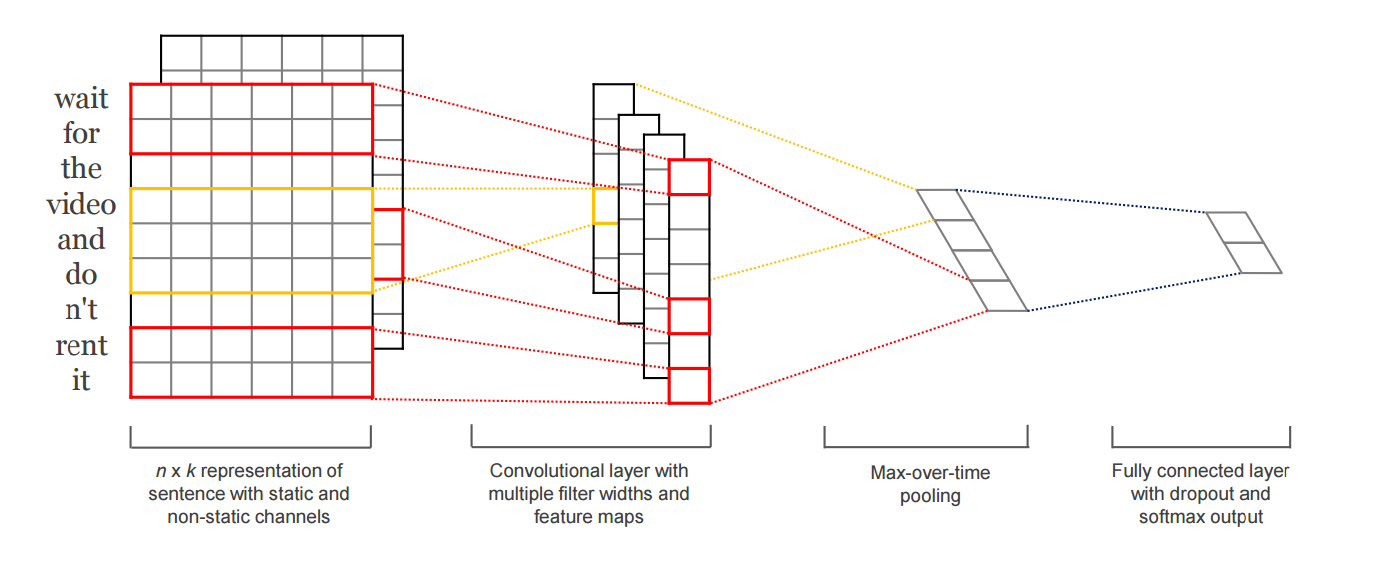
\includegraphics[width=12cm]{kimdiagram}
  \end{center}
  \begin{itemize}
  \item $n = 9$, $\dhid=4$ , $\dout=2$  
    \air 
  \item \alert{red}- $\dwin =2$, \structure{blue}- $\dwin =3$, (ignore back channel) 
    \air 

  \end{itemize}
\end{frame}

\begin{frame}{Classification Results}

  \begin{center}
    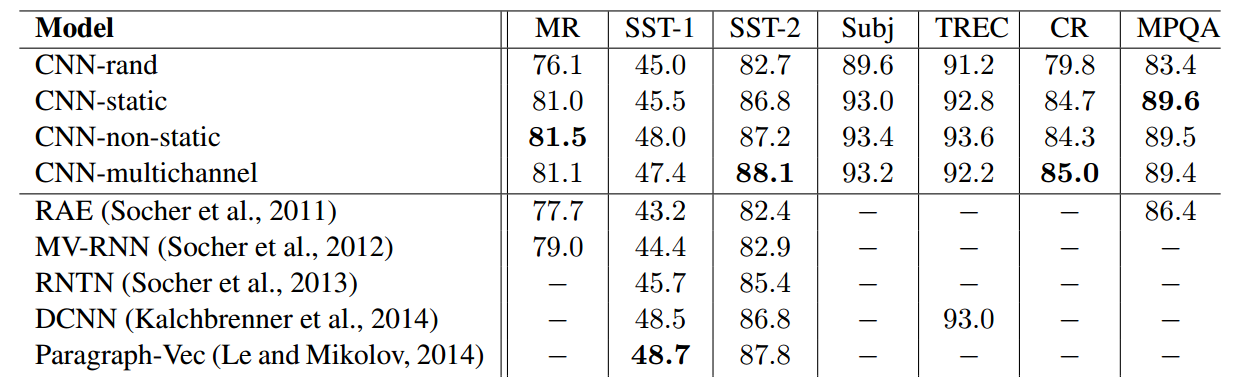
\includegraphics[width=12cm]{kimres}
  \end{center}
\end{frame}

\begin{frame}{Convolutional Vocabulary}
  \begin{itemize}
  \item \textbf{kernel size} or \textbf{filter width} ; window size $\dwin$
    \air 
  \item \textbf{filter}; column of matrix  $\boldW^1$ in $\reals^{(d^0\times \dwin)  \times 1}$  
    \air 

  \item \textbf{feature map}; column of $NN_{conv}$, $\dhid$ of these 
    \air 

  \item \textbf{fully-connected layer}; affine or linear  + activation  
    \air 

  \item \textbf{random}, \textbf{static}, \textbf{non-static}; embedding layer setup
    \air
  \item \textbf{temporal convolution}, \textbf{time-delay convolution}; names for one-dimensional convolutions
  \end{itemize}
\end{frame}

\begin{frame}{Why is it called a convolution?}

  \begin{itemize}
  \item Let $\boldx$ and $\boldy$ be in $\reals^n$ and $\reals^m$ 
  \end{itemize}
  
  \[[\boldx \ast \boldy]_i = \sum_{j=1}^m   x_{i-j} y_j\]
  
  \begin{itemize}
  \item Circular, $i-k$ wraps around. 
    \air 
  \item For NN, include padding
  \end{itemize}

  
\end{frame}


\section{Applications}


\begin{frame}{Language Applications: Semantic Role Labeling }
 He  would  n't accept anything of value from those he was writing about  

 \air 

 [A0 He ] [AM-MOD would ] [AM-NEG n't ] [V accept ] [A1 anything of value ] from [A2 those he was writing about ] 

\begin{itemize}
  \item V: verb 
   \item A0: acceptor 
   \item A1: thing accepted 
   \item A2: accepted-from 
   \item A3:attribute 
   \item AM-MOD: modal 
     \item  AM-NEG: negation
\end{itemize}
\end{frame}

\begin{frame}{Other Language Applications (Collobert et al. 2011) }
  \begin{center}
    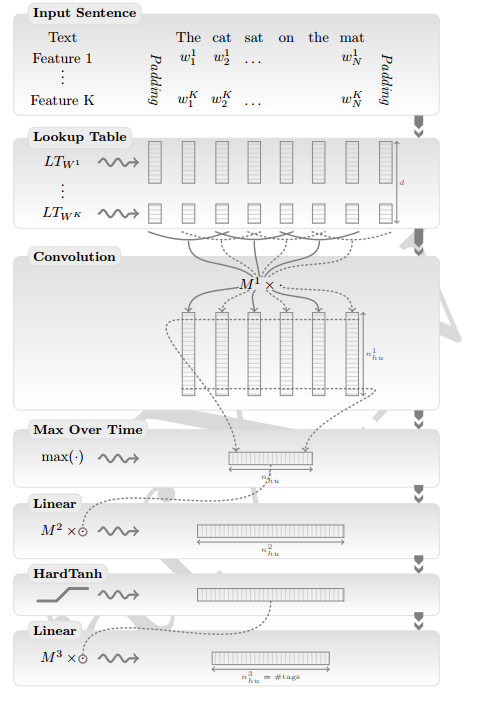
\includegraphics[width=5cm]{cwconv}
  \end{center}
\end{frame}

\begin{frame}{C\&W SRL }
  \begin{itemize}
  \item   First given a verb $w_i$ e.g. \texttt{accept}.
    \air 
  \item  Then consider a word $w_j$ e.g. \texttt{n't}
    \air
  \item  For a word $w_k$ features are 
    \[v(w_k), v_2(cap(w_k)), v_3(i-k), v_4(j-k)\]

    \air
  \item Convolution over sentence is used to predict role.
    \air 
  \item $O(n \times |verbs|)$ convolutions per sentence
  \end{itemize}
\end{frame}

{
\setbeamercolor{background canvas}{bg=}
\includepdf[pages=8]{aaai}
}

{
\setbeamercolor{background canvas}{bg=}
\includepdf[pages=16]{aaai}
}


{
\setbeamercolor{background canvas}{bg=}
\includepdf[pages=26-37]{aaai}
}

{
\setbeamercolor{background canvas}{bg=}
\includepdf[pages=63-66]{aaai}
}

{
\setbeamercolor{background canvas}{bg=}
\includepdf[pages=69-71]{aaai}
}

\section{Vision}
\begin{frame}{Visual Classification}
  \begin{center}
    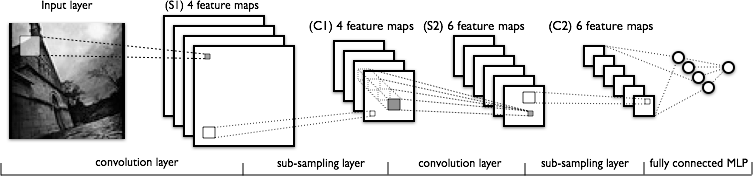
\includegraphics[width=\textwidth]{mylenet}
  \end{center}
\end{frame}


\begin{frame}{Speech Convolutions}
  \begin{center}
    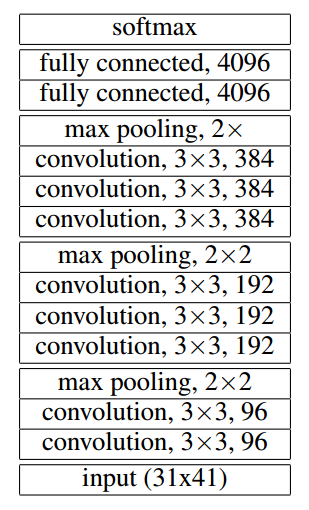
\includegraphics[width=5cm]{speechconv}
  \end{center}
  
\end{frame}

\begin{frame}{Visualization (Zeiler and Fergus, 2013)}
  \begin{center}
    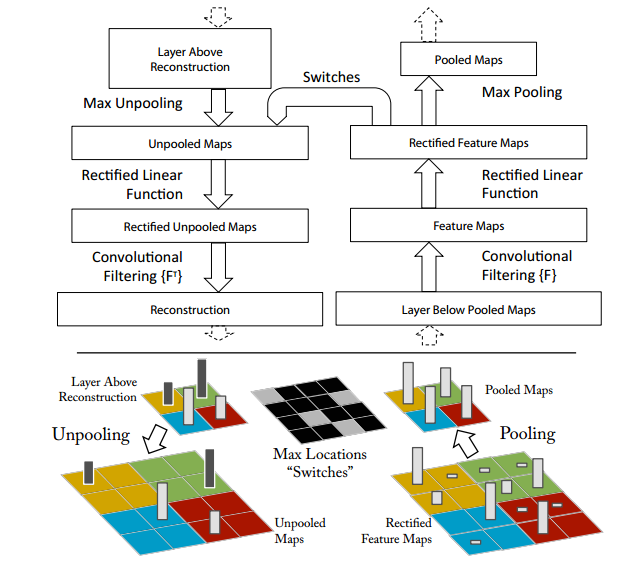
\includegraphics[height=\textheight]{zf}
  \end{center}
\end{frame}

\begin{frame}{Visualization (Zeiler and Fergus, 2013)}
  \begin{center}
    \includegraphics[height=\textheight]{filters}
  \end{center}
  
\end{frame}


\end{document}